\documentclass[14pt,a4paper]{extarticle}
% =============================================================
% preamble.tex — оформление отчётов по СТП БГУИР 01-2024
% =============================================================

% Шрифты: под pdflatex — Times через tempora + T2A,
% под xelatex/tectonic — системный Times New Roman (запасной вариант STIX Two Text)
\usepackage{iftex}
\ifPDFTeX
  \usepackage[utf8]{inputenc}
  \usepackage[T2A]{fontenc}
  \usepackage{tempora}
\else
  \usepackage{fontspec}
  \IfFontExistsTF{Times New Roman}
    {\setmainfont{Times New Roman}}
    {\setmainfont{STIX Two Text}}
  \IfFontExistsTF{DejaVu Sans Mono}
    {\setmonofont{DejaVu Sans Mono}[Scale=0.82]}
    {\setmonofont{DejaVuSansMono}[Extension=.ttf, BoldFont=*-Bold,
                                  ItalicFont=*-Oblique, Scale=0.82]}
\fi
\usepackage[russian]{babel}

% Поля: слева 30 мм, справа 15 мм, сверху и снизу 20 мм
\usepackage{geometry}
\geometry{left=30mm, right=15mm, top=20mm, bottom=20mm}

\usepackage{setspace}
\singlespacing

\pretolerance=1000
\tolerance=2000
\emergencystretch=3em

\usepackage{indentfirst}
\setlength{\parindent}{1.25cm}

% Номер страницы — снизу справа
\usepackage{fancyhdr}
\pagestyle{fancy}
\fancyhf{}
\fancyfoot[R]{\thepage}
\renewcommand{\headrulewidth}{0pt}
\fancypagestyle{plain}{%
  \fancyhf{}%
  \fancyfoot[R]{\thepage}%
  \renewcommand{\headrulewidth}{0pt}%
}

\usepackage{amsmath,amssymb}
\usepackage{graphicx}
\usepackage{float}
\usepackage{booktabs}
\usepackage{tabularx}
\usepackage{multirow}
\usepackage{longtable}
\usepackage{array}

\usepackage{caption}
\captionsetup[figure]{labelsep=endash, justification=centering,
                      font={normalsize}, name=Рисунок}
\captionsetup[table]{labelsep=endash, justification=raggedright,
                     singlelinecheck=false, font={normalsize}, name=Таблица}

\usepackage{titlesec}
\titleformat{\section}
  {\normalfont\fontsize{14}{18}\selectfont\bfseries}
  {\thesection}{0.5em}{\MakeUppercase}
\titlespacing*{\section}{1.25cm}{0pt}{14pt}
% Разрыв страницы до заголовка, чтобы номер в содержании совпадал со страницей раздела
\newcommand{\sectionbreak}{\clearpage}
\titleformat{\subsection}
  {\normalfont\fontsize{14}{18}\selectfont\bfseries}
  {\thesubsection}{0.5em}{}
\titlespacing*{\subsection}{1.25cm}{14pt}{14pt}
\titleformat{\subsubsection}
  {\normalfont\fontsize{14}{18}\selectfont\bfseries}
  {\thesubsubsection}{0.5em}{}
\titlespacing*{\subsubsection}{1.25cm}{14pt}{14pt}

\newcommand{\sectioncenter}[1]{%
  \newpage
  \phantomsection
  \addcontentsline{toc}{section}{#1}
  \begin{center}\textbf{\MakeUppercase{#1}}\end{center}
  \vspace{14pt}
}

\usepackage{tocloft}
\renewcommand{\cftsecfont}{\normalfont}
\renewcommand{\cftsecpagefont}{\normalfont}
\renewcommand{\cftsubsecfont}{\normalfont}
\renewcommand{\cftsubsecpagefont}{\normalfont}
\renewcommand{\cftsecleader}{\cftdotfill{\cftdotsep}}
\renewcommand{\cftdotsep}{1}
% babel переопределяет заголовки после преамбулы, поэтому правим через \addto
\addto\captionsrussian{\renewcommand{\contentsname}{\hfill\textbf{СОДЕРЖАНИЕ}\hfill}}
\renewcommand{\cftaftertoctitle}{\hfill}

\usepackage{enumitem}
\setlist[itemize]{noitemsep, topsep=0pt, leftmargin=1.25cm, label=--}
\setlist[enumerate]{noitemsep, topsep=0pt, leftmargin=1.25cm}

% Листинги кода и вывода программы
\usepackage{listings}
\usepackage{fancyvrb}
\lstset{
  basicstyle=\ttfamily\footnotesize,
  frame=single,
  breaklines=true,
  showstringspaces=false,
  inputencoding=utf8,
  extendedchars=true,
  columns=fullflexible,
  keepspaces=true,
  captionpos=t
}
\ifPDFTeX
\lstset{
  literate={а}{{\cyra}}1 {б}{{\cyrb}}1 {в}{{\cyrv}}1 {г}{{\cyrg}}1
           {д}{{\cyrd}}1 {е}{{\cyre}}1 {ж}{{\cyrzh}}1 {з}{{\cyrz}}1
           {и}{{\cyri}}1 {й}{{\cyrishrt}}1 {к}{{\cyrk}}1 {л}{{\cyrl}}1
           {м}{{\cyrm}}1 {н}{{\cyrn}}1 {о}{{\cyro}}1 {п}{{\cyrp}}1
           {р}{{\cyrr}}1 {с}{{\cyrs}}1 {т}{{\cyrt}}1 {у}{{\cyru}}1
           {ф}{{\cyrf}}1 {х}{{\cyrh}}1 {ц}{{\cyrc}}1 {ч}{{\cyrch}}1
           {ш}{{\cyrsh}}1 {щ}{{\cyrshch}}1 {ъ}{{\cyrhrdsn}}1
           {ы}{{\cyrery}}1 {ь}{{\cyrsftsn}}1 {э}{{\cyrerev}}1
           {ю}{{\cyryu}}1 {я}{{\cyrya}}1 {ё}{{\cyryo}}1
           {А}{{\CYRA}}1 {Б}{{\CYRB}}1 {В}{{\CYRV}}1 {Г}{{\CYRG}}1
           {Д}{{\CYRD}}1 {Е}{{\CYRE}}1 {Ж}{{\CYRZH}}1 {З}{{\CYRZ}}1
           {И}{{\CYRI}}1 {Й}{{\CYRISHRT}}1 {К}{{\CYRK}}1 {Л}{{\CYRL}}1
           {М}{{\CYRM}}1 {Н}{{\CYRN}}1 {О}{{\CYRO}}1 {П}{{\CYRP}}1
           {Р}{{\CYRR}}1 {С}{{\CYRS}}1 {Т}{{\CYRT}}1 {У}{{\CYRU}}1
           {Ф}{{\CYRF}}1 {Х}{{\CYRH}}1 {Ц}{{\CYRC}}1 {Ч}{{\CYRCH}}1
           {Ш}{{\CYRSH}}1 {Щ}{{\CYRSHCH}}1 {Ъ}{{\CYRHRDSN}}1
           {Ы}{{\CYRERY}}1 {Ь}{{\CYRSFTSN}}1 {Э}{{\CYREREV}}1
           {Ю}{{\CYRYU}}1 {Я}{{\CYRYA}}1 {Ё}{{\CYRYO}}1
           {—}{{---}}1 {–}{{--}}1 {…}{{\ldots}}1
}
\fi

% Подписи листингов — в том же стиле, что таблицы: «Листинг X.Y — Название»
\captionsetup[lstlisting]{labelsep=endash, justification=raggedright,
                          singlelinecheck=false, font={normalsize}}
\renewcommand{\lstlistingname}{Листинг}
\AtBeginDocument{\numberwithin{lstlisting}{section}}

\lstdefinestyle{python}{language=Python, keywordstyle=\bfseries}
\lstdefinestyle{shell}{language=bash, keywordstyle=\mdseries}
\lstdefinestyle{plain}{language={}, basicstyle=\ttfamily\scriptsize}

% Абзац после листинга должен сохранять отступ 1,25 см (СТП 2.1.1)
\makeatletter
\AtBeginDocument{\let\@endpetrue\@endpefalse}
\makeatother

% Подпись к блоку verbatim: \captionof вне плавающего окружения
% глобально обнуляет \parindent, поэтому отступ восстанавливается вручную
\newcommand{\listingcaption}[2]{%
  \captionof{lstlisting}{#1}\label{#2}%
  \setlength{\parindent}{1.25cm}%
}

\usepackage{hyperref}
\hypersetup{colorlinks=true, linkcolor=black, urlcolor=blue, citecolor=black}

\numberwithin{figure}{section}
\numberwithin{table}{section}
\numberwithin{equation}{section}

% Титульный лист отчёта по лабораторной работе
\newcommand{\makelabtitle}[2]{%
  \begin{titlepage}
  \thispagestyle{empty}
  \begin{center}

  МИНИСТЕРСТВО ОБРАЗОВАНИЯ РЕСПУБЛИКИ БЕЛАРУСЬ

  \vspace{0.5em}
  Учреждение образования

  \vspace{0.5em}
  \textbf{<<Белорусский государственный университет информатики и радиоэлектроники>>}

  \vspace{2em}
  Факультет компьютерных систем и сетей

  \vspace{0.5em}
  Кафедра программного обеспечения информационных технологий
  \end{center}

  \vspace{3em}
  \begin{center}
  \textbf{ОТЧЕТ}

  \vspace{0.5em}
  по лабораторной работе №#1

  \vspace{0.5em}
  по дисциплине

  \vspace{0.5em}
  <<Технологии компонентного программирования>>

  \vspace{0.5em}
  <<#2>>
  \end{center}

  \vspace{5em}
  \begin{flushright}
  \begin{minipage}{0.5\textwidth}
  \textbf{Выполнил:}\\
  Лебедевич Артем Владимирович\\
  магистрант группы 556301

  \vspace{0.6em}
  \textbf{Преподаватель:}\\
  Герман Олег Витольдович\\
  кандидат технических наук\\
  доцент кафедры ИТАС
  \end{minipage}
  \end{flushright}

  \vfill
  \begin{center}Минск, 2026~г.\end{center}
  \end{titlepage}
}


\newcolumntype{L}{>{\raggedright\arraybackslash}X}

\begin{document}

\makelabtitle{1}{Сериализация и десериализация объектов}

\tableofcontents

\section{Цель работы}

Изучить механизмы сериализации и десериализации объектов в языке Python. Создать класс
<<Студент>>, сохранить его объект в файл, восстановить в другом приложении, передать по
сети в клиент-серверном приложении, сериализовать состояние визуальной формы. Выполнить
все пункты отдельно для форматов pickle и JSON. Дополнительно передать вместе с объектом
изображение в формате WebP.

\section{Теоретические сведения}

\subsection{Сериализация и десериализация}

Сериализация --- преобразование объекта, существующего в памяти программы, в
последовательность байтов, которую можно записать в файл или передать по сети.
Десериализация --- обратное преобразование: по последовательности байтов строится
объект с теми же данными. Восстановленный объект является новым объектом, а не тем же
самым: совпадают значения полей, но не адрес в памяти.

Сериализация нужна, чтобы объект пережил границу процесса: для сохранения состояния
между запусками, обмена данными между программами и машинами, кэширования и постановки
сообщений в очереди. Она же лежит в основе компонентных технологий: при удалённом
вызове аргументы и результат метода передаются именно в сериализованном виде.

\subsection{Формат pickle}

Модуль \texttt{pickle} входит в стандартную библиотеку Python и сохраняет почти любые
объекты, включая экземпляры пользовательских классов. Формат двоичный, поэтому файлы
открываются в режимах \texttt{wb} и \texttt{rb}. Функции \texttt{dump} и
\texttt{dumps} преобразуют объект в байты, \texttt{load} и \texttt{loads} ---
обратно.

В поток записываются данные экземпляра и имя класса в виде <<модуль.класс>>, но не
код класса. Поэтому при восстановлении класс должен быть доступен для импорта, а методы
объекта берутся из этого класса. Формат понятен только Python и небезопасен:
десериализация данных из недоверенного источника может привести к выполнению
произвольного кода.

\subsection{Формат JSON}

JSON --- текстовый формат, который читается человеком и поддерживается всеми языками
программирования. Он знает только словари, списки, строки, числа, логические значения
и \texttt{null}, поэтому объект пользовательского класса нужно явно преобразовать в
словарь при записи и собрать обратно при чтении. Методы в JSON не попадают: они
появляются, когда из словаря создаётся объект класса.

Двоичные данные в JSON напрямую не записываются. Изображение кодируется в base64 ---
текстовое представление, в котором каждые три байта заменяются четырьмя символами,
поэтому объём растёт примерно на треть.

Сравнение форматов приведено в таблице~\ref{tab:formats}.

\begin{table}[H]
\caption{Сравнение форматов pickle и JSON}
\label{tab:formats}
\centering
\begin{tabularx}{\textwidth}{lLL}
\toprule
Свойство & pickle & JSON \\
\midrule
Вид данных & двоичный & текстовый \\
Пользовательские классы & сохраняются автоматически & нужно преобразование в
словарь \\
Изображение & исходные байты & строка base64 \\
Другие языки & только Python & любой язык \\
Безопасность & нельзя читать чужие данные & безопасен \\
\bottomrule
\end{tabularx}
\end{table}

\subsection{Передача по сети}

Протокол TCP передаёт поток байтов без границ сообщений: один вызов \texttt{recv} может
вернуть только часть отправленного. В примере из методических материалов используется
\texttt{recv(1024)}, чего достаточно для небольшого словаря, но не для объекта с
изображением. Поэтому в работе перед данными передаётся их длина, и получатель читает
ровно столько байтов, сколько объявлено. Формат сообщения показан в
таблице~\ref{tab:frame}.

\begin{table}[H]
\caption{Формат сообщения}
\label{tab:frame}
\centering
\begin{tabularx}{\textwidth}{llL}
\toprule
Поле & Размер & Содержимое \\
\midrule
Длина & 4 байта & длина остальной части, целое без знака, сетевой порядок байтов \\
Формат & 8 байт & строка \texttt{pickle} или \texttt{json}, дополненная нулями \\
Данные & переменный & сериализованный объект \\
\bottomrule
\end{tabularx}
\end{table}

\subsection{Сериализация визуальных объектов}

Элементы окна (кнопки, поля) связаны с ресурсами операционной системы и напрямую не
сериализуются. Сохраняется снимок состояния: заголовок окна, надпись на кнопке, текст
в поле ввода. По такому снимку окно создаётся заново --- этот же приём показан в
методических материалах на примере методов \texttt{to\_dict} и \texttt{from\_dict}.

\section{Реализация}

\subsection{Структура программы}

\listingcaption{Структура лабораторной работы}{lst:tree}
\begin{Verbatim}[fontsize=\footnotesize, frame=single, samepage=true]
lab1/models.py    классы Student, Photo и GuiFormState
lab1/codecs.py    сериализация в pickle и JSON, изображение в base64
lab1/net.py       сообщения с указанием длины
lab1/server.py    TCP-сервер: принимает объект и возвращает его
lab1/client.py    TCP-клиент: отправляет объект и читает ответ
lab1/reader.py    отдельное приложение, читающее файл с объектом
lab1/cases.py     проверяемые сценарии
lab1/gui.py       окно: карточка студента и список сценариев
lab1/gui_form.py  окно, восстановленное из снимка состояния
lab1/runner.py    запуск сценариев из командной строки
lab1/extras/      дополнительные задания
\end{Verbatim}

\subsection{Класс <<Студент>>}

Класс \texttt{Student} (листинг~\ref{lst:model}) содержит три поля из задания и
необязательную фотографию. Метод \texttt{greet} нужен, чтобы показать, что после
восстановления объект сохраняет поведение.

\begin{lstlisting}[style=python, caption={Классы предметной области}, label={lst:model}]
@dataclass
class Photo:
    filename: str
    mime: str
    data: bytes


@dataclass
class Student:
    name: str
    group: str
    faculty: str
    photo: Photo | None = None

    def greet(self) -> str:
        return f"{self.name}, {self.group}, {self.faculty}"
\end{lstlisting}

\subsection{Сериализация в pickle и JSON}

Для pickle достаточно вызова \texttt{pickle.dumps}: объект вместе с вложенной
фотографией сохраняется целиком, изображение --- как исходные байты. Для JSON написано
преобразование в словарь (листинг~\ref{lst:json}), где изображение кодируется в base64,
а рядом записываются имя файла и тип содержимого.

\begin{lstlisting}[style=python, caption={Преобразование объекта для JSON}, label={lst:json}]
def student_to_jsonable(student: Student) -> dict[str, Any]:
    payload: dict[str, Any] = {
        "name": student.name,
        "group": student.group,
        "faculty": student.faculty,
        "photo": None,
    }
    if student.photo is not None:
        payload["photo"] = {
            "filename": student.photo.filename,
            "mime": student.photo.mime,
            "encoding": "base64",
            "data": base64.b64encode(student.photo.data).decode("ascii"),
        }
    return payload
\end{lstlisting}

\subsection{Десериализация в другом приложении}

Модуль \texttt{lab1/reader.py} запускается отдельным процессом командой
\texttt{python -m lab1.reader artifacts/student.json}. Он определяет формат по
расширению файла, восстанавливает объект и вызывает его метод. Для файла pickle при
этом проверяется, что получен именно объект класса \texttt{Student}.

\subsection{Клиент-серверное приложение}

Функции приёма и передачи сообщений приведены в листинге~\ref{lst:net}. Функция
\texttt{recv\_exact} читает из сокета в цикле, пока не получит заданное число байтов,
и тем самым устраняет ограничение в 1024~байта. Сервер восстанавливает объект,
передаёт его в окно программы и возвращает клиенту то же сообщение; клиент
восстанавливает объект из ответа.

\begin{lstlisting}[style=python, caption={Сообщения с указанием длины}, label={lst:net}]
HEADER = struct.Struct("!I")


def send_message(sock: socket.socket, payload: bytes) -> None:
    if len(payload) > MAX_PAYLOAD:
        raise ValueError(f"payload too large: {len(payload)} bytes")
    sock.sendall(HEADER.pack(len(payload)) + payload)


def recv_exact(sock: socket.socket, size: int) -> bytes:
    chunks = bytearray()
    while len(chunks) < size:
        piece = sock.recv(size - len(chunks))
        if not piece:
            raise ConnectionError("socket closed while reading")
        chunks.extend(piece)
    return bytes(chunks)


def recv_message(sock: socket.socket) -> bytes:
    (length,) = HEADER.unpack(recv_exact(sock, HEADER.size))
    if length > MAX_PAYLOAD:
        raise ValueError(f"declared payload too large: {length}")
    return recv_exact(sock, length)
\end{lstlisting}

\subsection{Сериализация визуальной формы}

Состояние формы с кнопкой и текстовым полем описывается классом
\texttt{GuiFormState} (листинг~\ref{lst:form}). Снимок записывается в файл
\texttt{artifacts/gui\_form.json}, после чего по нему открывается новое окно.

\begin{lstlisting}[style=python, caption={Снимок состояния визуальной формы}, label={lst:form}]
@dataclass
class GuiFormState:
    title: str = "Visual form"
    button_label: str = "Click me"
    text_value: str = ""
    label_text: str = "Welcome"
    extra: dict[str, str] = field(default_factory=dict)

    def to_dict(self) -> dict[str, object]:
        return {
            "title": self.title,
            "button_label": self.button_label,
            "text_value": self.text_value,
            "label_text": self.label_text,
            "extra": self.extra,
        }
\end{lstlisting}

\subsection{Графическое приложение}

Окно написано на библиотеке wxPython. Слева находится карточка студента с полями и
фотографией, справа --- список сценариев, каждый из которых соответствует пункту
задания и запускается кнопкой Run либо все сразу кнопкой All. Изображение WebP для
предварительного просмотра декодируется библиотекой Pillow.

\section{Дополнительные задания}

Три дополнительные темы выполнены как продолжение работы и размещены в каталоге
\texttt{lab1/extras}.

\subsection{Удалённый вызов модуля}

В каталоге \texttt{lab1/extras/rpc} реализован сервер XML-RPC на основе стандартного
класса \texttt{SimpleXMLRPCServer} с методами \texttt{add}, \texttt{mul},
\texttt{greet\_student} и \texttt{inspect\_module}. Клиентов два: на Python
(\texttt{xmlrpc.client}) и на Java без сторонних библиотек. Связь с основной работой
прямая: при удалённом вызове аргументы и результат сериализуются в XML автоматически.
Окно показано на рисунке~\ref{fig:rpc}.

\begin{figure}[H]
\centering
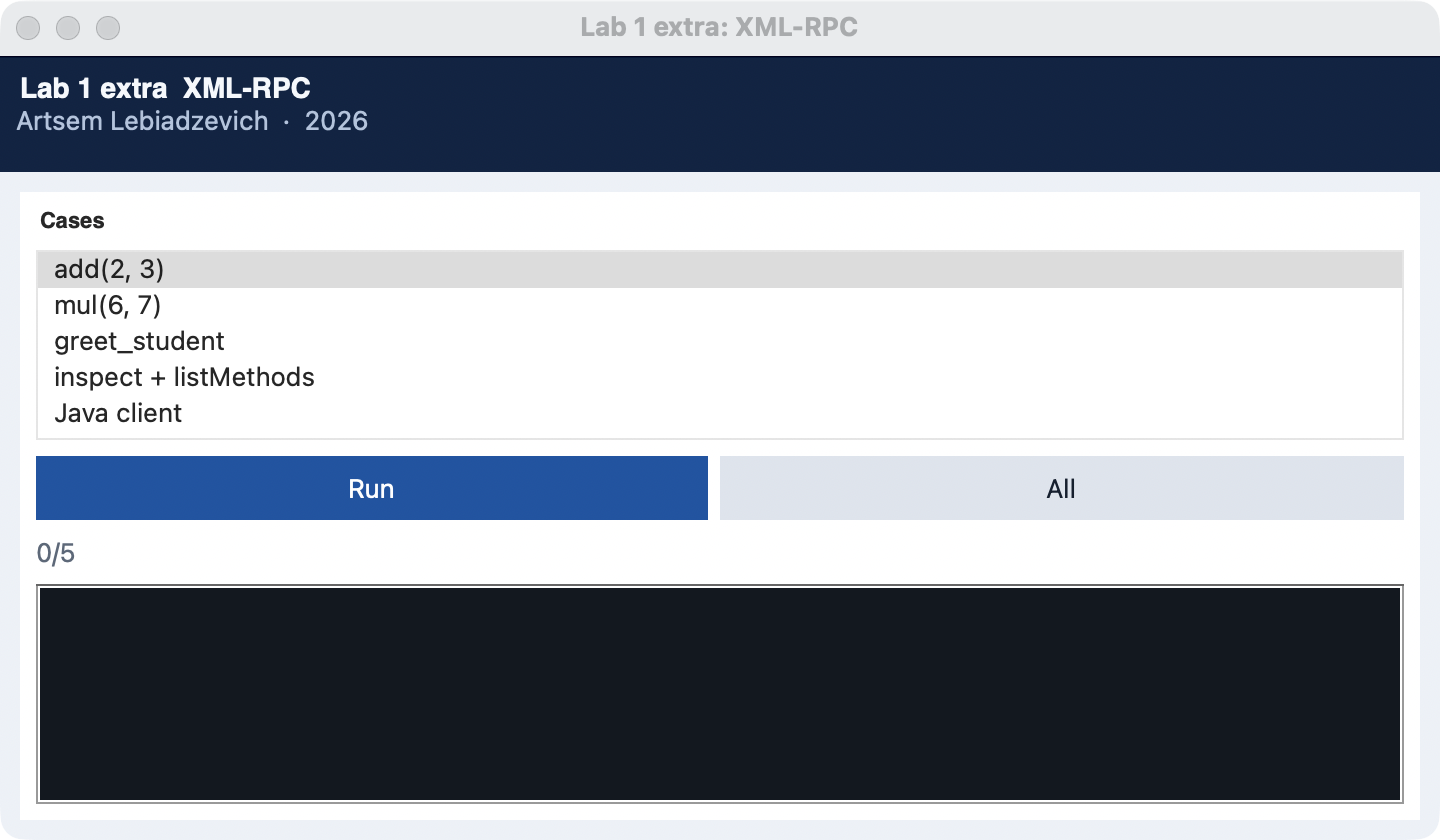
\includegraphics[width=0.75\textwidth]{../screenshots/lab1_extra_rpc.png}
\caption{Дополнительное задание: удалённый вызов через XML-RPC}
\label{fig:rpc}
\end{figure}

\subsection{Компоненты wxPython}

В каталоге \texttt{lab1/extras/wxui} собрано окно с панелью инструментов: просмотр
изображения, проигрывание звука, встроенный браузер, календарь с часами, чтение PDF,
запуск Word и Excel, а также собственный компонент \texttt{CustomButton} ---
наследник стандартной кнопки. Общие элементы оформления из этого задания используются
всеми окнами лабораторных работ.

\subsection{Рефлексия}

В каталоге \texttt{lab1/extras/reflection} класс \texttt{Student} создаётся во время
выполнения функцией \texttt{type}, его методы и сигнатуры исследуются модулем
\texttt{inspect}, новые методы добавляются объекту через \texttt{types.MethodType}.
Программа на Java передаёт имя метода строкой, а Python находит и вызывает его функцией
\texttt{getattr}. Окно показано на рисунке~\ref{fig:reflection}.

\begin{figure}[H]
\centering
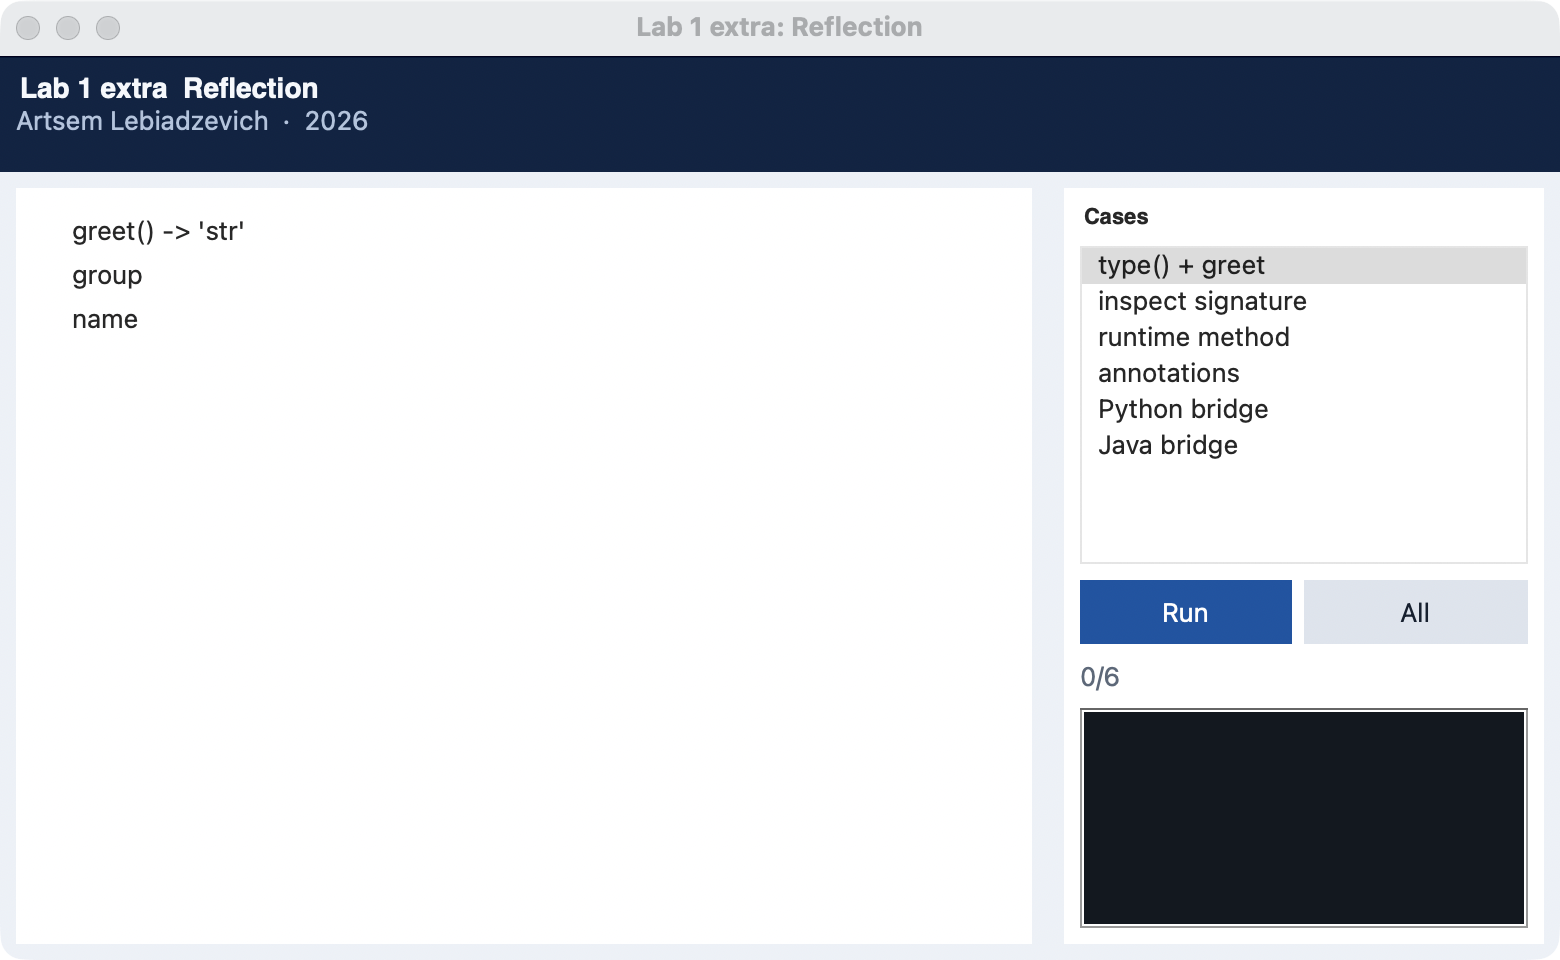
\includegraphics[width=0.75\textwidth]{../screenshots/lab1_extra_reflection.png}
\caption{Дополнительное задание: рефлексия}
\label{fig:reflection}
\end{figure}

\section{Результаты работы программы}

Окно запускается командой \texttt{python main.py -{}-lab 1 -{}-gui}
(рисунок~\ref{fig:lab1}). В журнале справа видно, что объект с фотографией размером
6122~байта записан в оба формата, прочитан другим процессом и передан по сети без
потерь.

\begin{figure}[H]
\centering
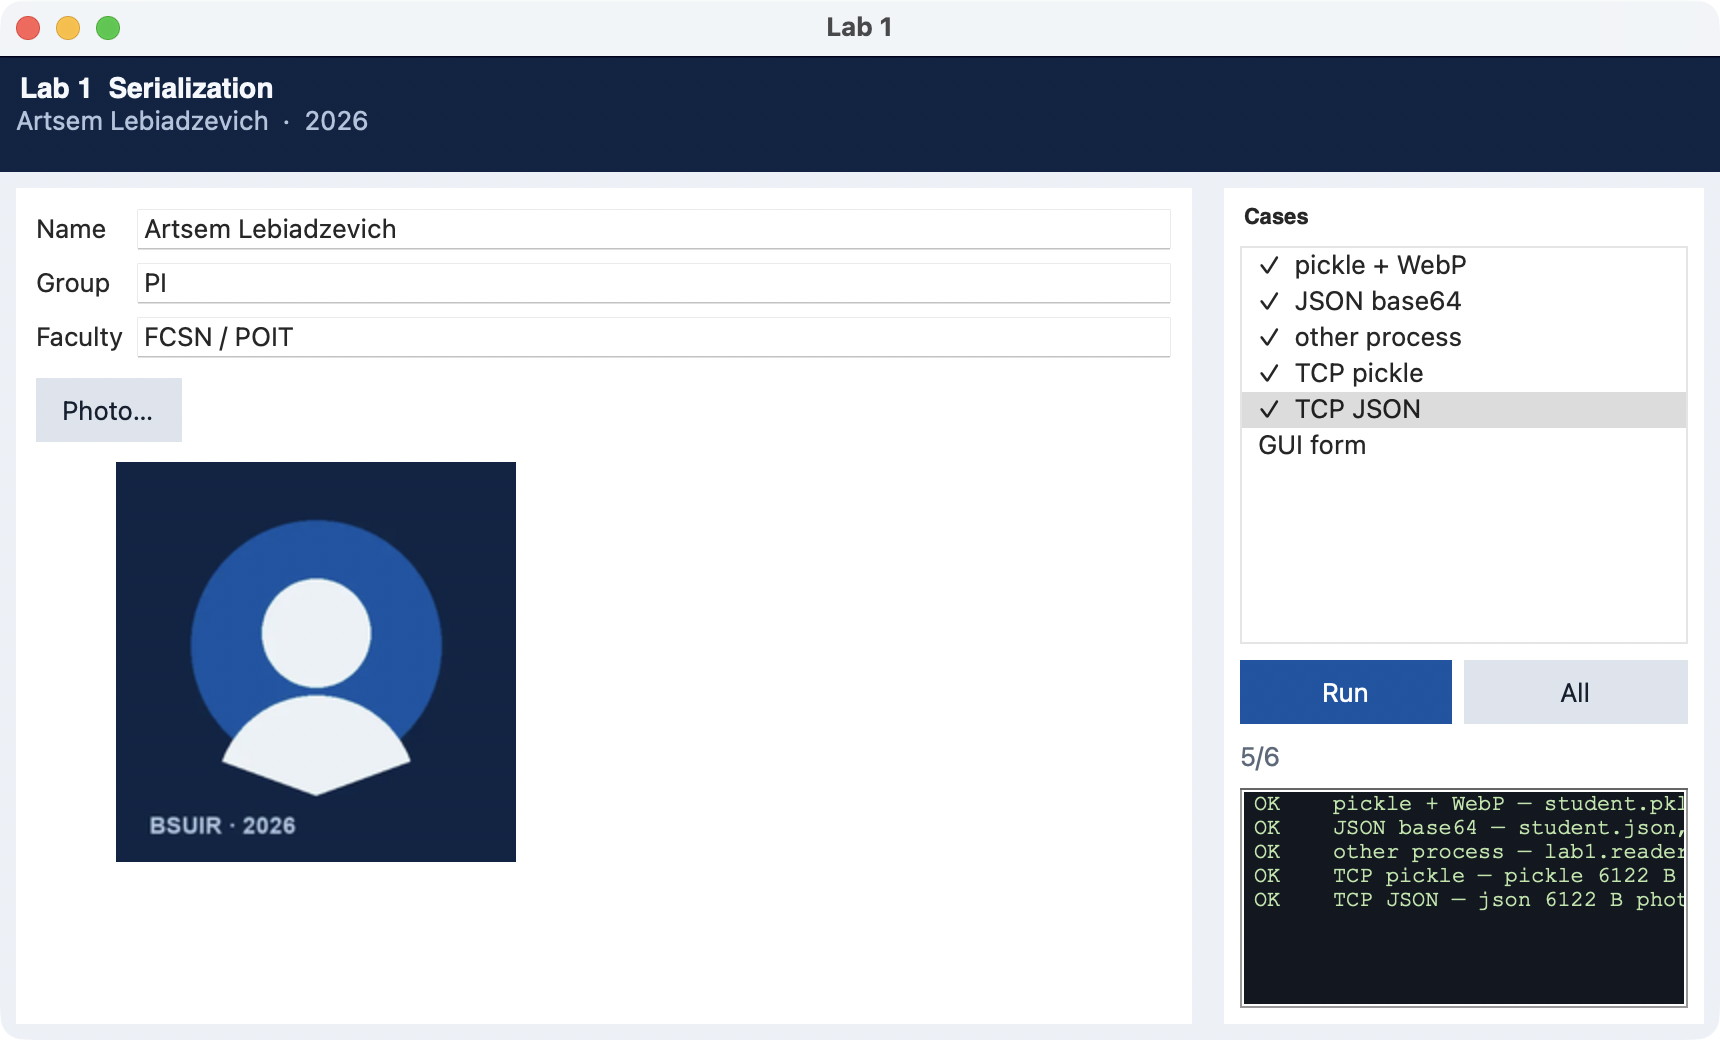
\includegraphics[width=0.9\textwidth]{../screenshots/lab1.png}
\caption{Окно лабораторной работы после выполнения сценариев}
\label{fig:lab1}
\end{figure}

Команда \texttt{python main.py -{}-lab 1} выполняет те же действия без окна
(листинг~\ref{lst:cli}).

\lstinputlisting[style=plain, caption={Вывод программы}, label={lst:cli}]{listings/cli_output.txt}

Файл pickle занимает 6320~байт, файл JSON --- 8360~байт при размере изображения
6122~байта: разница объясняется кодированием base64. Соответствие пунктам задания
приведено в таблице~\ref{tab:results}.

\begin{table}[H]
\caption{Выполнение пунктов задания}
\label{tab:results}
\centering
\small
\begin{tabularx}{\textwidth}{c>{\raggedright\arraybackslash}p{6cm}L}
\toprule
Пункт & Задание & Где выполнено \\
\midrule
1 & класс <<Студент>> & \texttt{lab1/models.py} \\
2 & создание объекта & окно и \texttt{lab1/runner.py} \\
3 & сериализация в двоичный файл & \texttt{artifacts/student.pkl} \\
4 & десериализация в другом приложении & \texttt{python -m lab1.reader} \\
5 & передача по сети & \texttt{lab1/server.py}, \texttt{lab1/client.py} \\
6 & десериализация на принимающей стороне & сервер и клиент восстанавливают объект \\
7 & визуальный объект & \texttt{GuiFormState}, \texttt{artifacts/\allowbreak gui\_form.json} \\
8 & pickle и JSON отдельно & сценарии для каждого формата \\
\bottomrule
\end{tabularx}
\end{table}

Автоматические тесты проверяют совпадение байтов изображения после восстановления из
pickle и из JSON, передачу сообщения длиной 5000~байт, превышающей 1024~байта, и ответ
сервера. Все тесты проходят.

\section{Ответы на контрольные вопросы}

\textbf{1. Что такое сериализация и десериализация?} Сериализация --- преобразование
объекта в последовательность байтов для хранения или передачи. Десериализация ---
восстановление объекта из этой последовательности.

\textbf{2. Какие платформы используются для сериализации?} В Python --- модули
\texttt{pickle}, \texttt{json} и \texttt{marshal}. В других средах применяются
\texttt{Serializable} в Java, \texttt{System.Text.Json} в .NET, а также независимые
от языка форматы XML и Protocol Buffers.

\textbf{3. В чём польза сериализации?} Она позволяет сохранять состояние программы,
обмениваться объектами между процессами и машинами, кэшировать результаты и передавать
сообщения. На ней основаны удалённые вызовы и компонентные технологии.

\textbf{4. Можно ли сериализовать объект, у которого есть методы?} Да. Формат pickle
сохраняет данные объекта и имя класса, а методы после восстановления берутся из
класса, который должен быть доступен принимающей программе. В JSON попадают только
данные; методы появляются, когда из словаря создаётся объект класса.

\sectioncenter{Заключение}

В ходе лабораторной работы изучены сериализация и десериализация объектов и выполнены
все пункты задания для форматов pickle и JSON: объект класса <<Студент>> сохранён в
файл, восстановлен отдельным приложением, передан по сети и восстановлен на принимающей
стороне, а состояние визуальной формы сохранено и использовано для создания нового
окна. Дополнительно вместе с объектом передаётся изображение WebP.

Практические выводы работы следующие. Формат pickle удобен внутри одной программы на
Python, но не годится для обмена с другими языками и недоверенными источниками; на
границе систем применяется JSON, где двоичные данные требуют base64 и увеличивают объём
примерно на треть. При передаче по TCP длину сообщения нужно указывать явно, иначе
объект, не поместившийся в один вызов \texttt{recv}, будет получен не полностью.
Сериализация является основой следующих тем курса: удалённого вызова и компонентных
технологий, где через границу процесса передаётся уже не объект, а вызов его метода.

\sectioncenter{Список использованных источников}

\begin{enumerate}
\item Герман, О.~В. Сериализация и десериализация: лекция и лабораторная работа по
дисциплине <<Технологии компонентного программирования>> / О.~В.~Герман. --- Минск:
БГУИР, 2024.
\item Лутц, М. Программирование на Python: в 2~т. / М.~Лутц. --- 4-е изд. --- СПб.:
Символ-Плюс, 2011. --- Т.~2. --- 992~с.
\item Python documentation. pickle --- Python object serialization [Электронный
ресурс]. --- Режим доступа: \url{https://docs.python.org/3/library/pickle.html}.
\item Python documentation. json --- JSON encoder and decoder [Электронный ресурс]. ---
Режим доступа: \url{https://docs.python.org/3/library/json.html}.
\end{enumerate}

\end{document}
